\documentclass[conference,compsoc]{IEEEtran}
% Some/most Computer Society conferences require the compsoc mode option,
% but others may want the standard conference format.
%
% If IEEEtran.cls has not been installed into the LaTeX system files,
% manually specify the path to it like:
% \documentclass[conference,compsoc]{../sty/IEEEtran}



% Some very useful LaTeX packages include:
% (uncomment the ones you want to load)


% *** MISC UTILITY PACKAGES ***
\usepackage{graphicx}
\usepackage{amsmath,amssymb}
\usepackage{changepage}
\DeclareMathOperator{\E}{\mathbb{E}}

%\usepackage{ifpdf}
% Heiko Oberdiek's ifpdf.sty is very useful if you need conditional
% compilation based on whether the output is pdf or dvi.
% usage:
% \ifpdf
%   % pdf code
% \else
%   % dvi code
% \fi
% The latest version of ifpdf.sty can be obtained from:
% http://www.ctan.org/pkg/ifpdf
% Also, note that IEEEtran.cls V1.7 and later provides a builtin
% \ifCLASSINFOpdf conditional that works the same way.
% When switching from latex to pdflatex and vice-versa, the compiler may
% have to be run twice to clear warning/error messages.






% *** CITATION PACKAGES ***
%
\ifCLASSOPTIONcompsoc
  % IEEE Computer Society needs nocompress option
  % requires cite.sty v4.0 or later (November 2003)
  \usepackage[nocompress]{cite}
\else
  % normal IEEE
  \usepackage{cite}
\fi

% correct bad hyphenation here
\hyphenation{op-tical net-works semi-conduc-tor}


\begin{document}
%
% paper title
% Titles are generally capitalized except for words such as a, an, and, as,
% at, but, by, for, in, nor, of, on, or, the, to and up, which are usually
% not capitalized unless they are the first or last word of the title.
% Linebreaks \\ can be used within to get better formatting as desired.
% Do not put math or special symbols in the title.
\title{Neural Network solutions to Witsenhausen problem}


% author names and affiliations
% use a multiple column layout for up to three different
% affiliations
\author{\IEEEauthorblockN{Jiaojiao Fan}
\IEEEauthorblockA{GTID:903565753\\ Email: jiaojiaofan@gatech.edu}}


% make the title area
\maketitle

% As a general rule, do not put math, special symbols or citations
% in the abstract
\begin{abstract}
 In this report, several neural networks with different structures are implemented to solve Witsenhausen problem. Other improving strategies include optimizers, initializations and forced function fixing. Finally, the result are compared with former people and a better result is obtained. Also, the shortcoming of the neural network also shows in this project. The neural network may be stuck into a near local minima.
\end{abstract}


\section{Introduction}
  In this report, we proposed several solutions to the well-known and still unsolved Witsenhausen counterexample. \cite{witsenhausen1968counterexample} There have been some meaningful tries to detect the global minima of the min problem, such as Lee \cite{lee2001witsenhausen}and M. Barglietto \cite{baglietto2001numerical} Some of their manipulations are also refered in this project. Other than that, thanks to the development of the neural networks, many other meaningful attempts are also taken such as input convex neural network (ICNN) structure \cite{amos2017input} Different results would be listed to show the effect.

% You must have at least 2 lines in the paragraph with the drop letter
% (should never be an issue)

% \subsection{Subsection Heading Herex1}
% Subsection text here.


% \subsubsection{Subsubsection Heading Here}
% Subsubsection text here.


% An example of a floating figure using the graphicx package.
% Note that \label must occur AFTER (or within) \caption.
% For figures, \caption should occur after the \includegraphics.
% Note that IEEEtran v1.7 and later has special internal code that
% is designed to preserve the operation of \label within \caption
% even when the captionsoff option is in effect. However, because
% of issues like this, it may be the safest practice to put all your
% \label just after \caption rather than within \caption{}.
%
% Reminder: the "draftcls" or "draftclsnofoot", not "draft", class
% option should be used if it is desired that the figures are to be
% displayed while in draft mode.
%
%\begin{figure}[!t]
%\centering
%\includegraphics[width=2.5in]{myfigure}
% where an .eps filename suffix will be assumed under latex, 
% and a .pdf suffix will be assumed for pdflatex; or what has been declared
% via \DeclareGraphicsExtensions.
%\caption{Simulation results for the network.}
%\label{fig_sim}
%\end{figure}

% Note that the IEEE typically puts floats only at the top, even when this
% results in a large percentage of a column being occupied by floats.


% An example of a double column floating figure using two subfigures.
% (The subfig.sty package must be loaded for this to work.)
% The subfigure \label commands are set within each subfloat command,
% and the \label for the overall figure must come after \caption.
% \hfil is used as a separator to get equal spacing.
% Watch out that the combined width of all the subfigures on a 
% line do not exceed the text width or a line break will occur.
%
%\begin{figure*}[!t]
%\centering
%\subfloat[Case I]{\includegraphics[width=2.5in]{box}%
%\label{fig_first_case}}
%\hfil
%\subfloat[Case II]{\includegraphics[width=2.5in]{box}%
%\label{fig_second_case}}
%\caption{Simulation results for the network.}
%\label{fig_sim}
%\end{figure*}
%
% Note that often IEEE papers with subfigures do not employ subfigure
% captions (using the optional argument to \subfloat[]), but instead will
% reference/describe all of them (a), (b), etc., within the main caption.
% Be aware that for subfig.sty to generate the (a), (b), etc., subfigure
% labels, the optional argument to \subfloat must be present. If a
% subcaption is not desired, just leave its contents blank,
% e.g., \subfloat[].


% An example of a floating table. Note that, for IEEE style tables, the
% \caption command should come BEFORE the table and, given that table
% captions serve much like titles, are usually capitalized except for words
% such as a, an, and, as, at, but, by, for, in, nor, of, on, or, the, to
% and up, which are usually not capitalized unless they are the first or
% last word of the caption. Table text will default to \footnotesize as
% the IEEE normally uses this smaller font for tables.
% The \label must come after \caption as always.
%
%\begin{table}[!t]
%% increase table row spacing, adjust to taste
%\renewcommand{\arraystretch}{1.3}
% if using array.sty, it might be a good idea to tweak the value of
% \extrarowheight as needed to properly center the text within the cells
%\caption{An Example of a Table}
%\label{table_example}
%\centering
%% Some packages, such as MDW tools, offer better commands for making tables
%% than the plain LaTeX2e tabular which is used here.
%\begin{tabular}{|c||c|}
%\hline
%One & Two\\
%\hline
%Three & Four\\
%\hline
%\end{tabular}
%\end{table}


% Note that the IEEE does not put floats in the very first column
% - or typically anywhere on the first page for that matter. Also,
% in-text middle ("here") positioning is typically not used, but it
% is allowed and encouraged for Computer Society conferences (but
% not Computer Society journals). Most IEEE journals/conferences use
% top floats exclusively. 
% Note that, LaTeX2e, unlike IEEE journals/conferences, places
% footnotes above bottom floats. This can be corrected via the
% \fnbelowfloat command of the stfloats package.


\section{The Witsenhausen Counterexample}

The Witsenhausen counterexample has been outstanding for more than 50 years. It is formulated by Hans Witsenhausen in 1968.\cite{witsenhausen1968counterexample} It is a counterexample to a natural conjecture that in a system with linear dynamics, Gaussian disturbance, and quadratic cost,affine control laws are optimal to minimize the cost. However, Witsenhausen courterexample, shown in figure below,
\begin{figure}[htp]
    \centering
    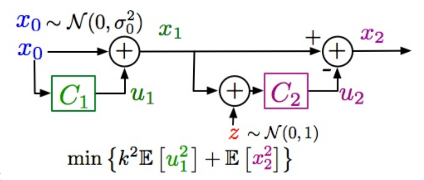
\includegraphics[width=6cm]{images/Wits_definition.png}
    \caption{Witsenhausen couterexample}
    \label{fig:definition}
\end{figure}
has nonlinear control laws that outperform all linear laws.
\begin{equation}
    f(x)=\gamma_1(x)+x \hspace{1cm} g(x)=\gamma_2(x)
\end{equation}

As a result, $f(x_0)=x_1$ and $g(x_1+z)=u_2$. Out goal is to minimize the quadratic cost:$k^{2} \E [U_1^{2}]+\E[X_2^{2}]$, which can also be written as 
\begin{equation}\label{eq:minJ}
\begin{aligned}
\mathrm{min}J(f,g):=&k^{2}\E[f(X_0)-X_0]^{2}+\\
&\E[(f(X_0)-g(f(X_0)+N))^{2}]
\end{aligned}
\end{equation}

In equation \eqref{eq:minJ}, there is a parameter $k^2$, which in fact determines the cost gap between the linear controller and nonlinear controller\cite{baglietto2001numerical}. If $k^2$ is smaller, the gap is bigger. For better comparison with the results got by previous researchers, $k^2$ is set as 0.04 in this report.

In addition, it is already known that $f(x)$ must have some strict property to be optimal \cite{wu2011witsenhausen} :
\begin{adjustwidth}{0.5cm}{}
\textbullet \quad \textit{Any optimal controller f is a strictly increasing unbounded piecewise real analytic function with a real analytic inverse}
\end{adjustwidth}

This means $f$ has to be smooth enough. But interestingly, the neural network(NN) optimized result is exactly opposite from this property. The sharper the $f$ becomes (opposite to smooth), the smaller the cost is.

\section{Basic Neural Network Setup}
The whold process could be generally separated into 4 parts:\\
1) Initialization setup for the $f$ net and $g$ net\\
2) Train the NNs using Gaussian distribution data. In this report, all data keeps the consistency: $x_0\sim N(0,\sigma^2)$ and $\sigma=5$, 

\subsection{Neural Network Architecture}
 Basically, two NNs are taken to represent $f$ and $g$ seperately using Pytorch structure. \footnote{The code of this project could be found at: https://github.com/sbyebss/Witsenhausen}
For $f$ net, all layers are linear layers and CELU\cite{barron2017continuously} activation function is used since it makes the activation function continuously differentiable and improves the performance in initialization setup process.

% use section* for acknowledgment
\section*{Acknowledgment}
Thanks to my advisor: Dr. Yongxin Chen and the other PhD studens: Rahul Singh and Qinsheng Zhang for their kind help. They give me a lot of ideas about how to improve the performance during the process of project.
% trigger a \newpage just before the given reference
% number - used to balance the columns on the last page
% adjust value as needed - may need to be readjusted if
% the document is modified later
%\IEEEtriggeratref{8}
% The "triggered" command can be changed if desired:
%\IEEEtriggercmd{\enlargethispage{-5in}}

% references section
\bibliographystyle{IEEEtran}
\bibliography{annot_report}

\end{document}


